%%%%%%%%%%%%%%%%%%%%%%%%%%%%%%%%%%%%%%%%%
% Beamer Presentation
% LaTeX Template
% Version 2.0 (March 8, 2022)
%
% This template originates from:
% https://www.LaTeXTemplates.com
%
% Author:
% Vel (vel@latextemplates.com)
%
% License:
% CC BY-NC-SA 4.0 (https://creativecommons.org/licenses/by-nc-sa/4.0/)
%
%%%%%%%%%%%%%%%%%%%%%%%%%%%%%%%%%%%%%%%%%

%----------------------------------------------------------------------------------------
%	PACKAGES AND OTHER DOCUMENT CONFIGURATIONS
%----------------------------------------------------------------------------------------

\documentclass[
	9pt, % Set the default font size, options include: 8pt, 9pt, 10pt, 11pt, 12pt, 14pt, 17pt, 20pt
	%t, % Uncomment to vertically align all slide content to the top of the slide, rather than the default centered
	%aspectratio=169, % Uncomment to set the aspect ratio to a 16:9 ratio which matches the aspect ratio of 1080p and 4K screens and projectors
]{beamer}

\graphicspath{{Images/}{./}} % Specifies where to look for included images (trailing slash required)

\usepackage{booktabs} % Allows the use of \toprule, \midrule and \bottomrule for better rules in tables
\usepackage{bm}
\usepackage{graphicx}
\usepackage{float}
\usepackage{subfigure}
%\usepackage{caption2}
\usepackage{amsmath}

%----------------------------------------------------------------------------------------
%	SELECT LAYOUT THEME
%----------------------------------------------------------------------------------------

% Beamer comes with a number of default layout themes which change the colors and layouts of slides. Below is a list of all themes available, uncomment each in turn to see what they look like.

%\usetheme{default}
\usetheme{AnnArbor}
%\usetheme{Antibes}
%\usetheme{Bergen}
%\usetheme{Berkeley}
%\usetheme{Berlin}
%\usetheme{Boadilla}
%\usetheme{CambridgeUS}
%\usetheme{Copenhagen}
%\usetheme{Darmstadt}
%\usetheme{Dresden}
%\usetheme{Frankfurt}
%\usetheme{Goettingen}
%\usetheme{Hannover}
%\usetheme{Ilmenau}
%\usetheme{JuanLesPins}
%\usetheme{Luebeck}
%\usetheme{Madrid}
%\usetheme{Malmoe}
%\usetheme{Marburg}
%\usetheme{Montpellier}
%\usetheme{PaloAlto}
%\usetheme{Pittsburgh}
%\usetheme{Rochester}
%\usetheme{Singapore}
%\usetheme{Szeged}
%\usetheme{Warsaw}

%----------------------------------------------------------------------------------------
%	SELECT COLOR THEME
%----------------------------------------------------------------------------------------

% Beamer comes with a number of color themes that can be applied to any layout theme to change its colors. Uncomment each of these in turn to see how they change the colors of your selected layout theme.

%\usecolortheme{albatross}
%\usecolortheme{beaver}
%\usecolortheme{beetle}
%\usecolortheme{crane}
%\usecolortheme{dolphin}
%\usecolortheme{dove}
%\usecolortheme{fly}
%\usecolortheme{lily}
%\usecolortheme{monarca}
%\usecolortheme{seagull}
%\usecolortheme{seahorse}
%\usecolortheme{spruce}
%\usecolortheme{whale}
%\usecolortheme{wolverine}

%----------------------------------------------------------------------------------------
%	SELECT FONT THEME & FONTS
%----------------------------------------------------------------------------------------

% Beamer comes with several font themes to easily change the fonts used in various parts of the presentation. Review the comments beside each one to decide if you would like to use it. Note that additional options can be specified for several of these font themes, consult the beamer documentation for more information.

\usefonttheme{default} % Typeset using the default sans serif font
%\usefonttheme{serif} % Typeset using the default serif font (make sure a sans font isn't being set as the default font if you use this option!)
%\usefonttheme{structurebold} % Typeset important structure text (titles, headlines, footlines, sidebar, etc) in bold
%\usefonttheme{structureitalicserif} % Typeset important structure text (titles, headlines, footlines, sidebar, etc) in italic serif
%\usefonttheme{structuresmallcapsserif} % Typeset important structure text (titles, headlines, footlines, sidebar, etc) in small caps serif

%------------------------------------------------

%\usepackage{mathptmx} % Use the Times font for serif text
\usepackage{palatino} % Use the Palatino font for serif text

%\usepackage{helvet} % Use the Helvetica font for sans serif text
\usepackage[default]{opensans} % Use the Open Sans font for sans serif text
%\usepackage[default]{FiraSans} % Use the Fira Sans font for sans serif text
%\usepackage[default]{lato} % Use the Lato font for sans serif text

%----------------------------------------------------------------------------------------
%	SELECT INNER THEME
%----------------------------------------------------------------------------------------

% Inner themes change the styling of internal slide elements, for example: bullet points, blocks, bibliography entries, title pages, theorems, etc. Uncomment each theme in turn to see what changes it makes to your presentation.

%\useinnertheme{default}
\useinnertheme{circles}
%\useinnertheme{rectangles}
%\useinnertheme{rounded}
%\useinnertheme{inmargin}

%----------------------------------------------------------------------------------------
%	SELECT OUTER THEME
%----------------------------------------------------------------------------------------

% Outer themes change the overall layout of slides, such as: header and footer lines, sidebars and slide titles. Uncomment each theme in turn to see what changes it makes to your presentation.

%\useoutertheme{default}
%\useoutertheme{infolines}
%\useoutertheme{miniframes}
%\useoutertheme{smoothbars}
%\useoutertheme{sidebar}
%\useoutertheme{split}
%\useoutertheme{shadow}
%\useoutertheme{tree}
%\useoutertheme{smoothtree}

%\setbeamertemplate{footline} % Uncomment this line to remove the footer line in all slides
%\setbeamertemplate{footline}[page number] % Uncomment this line to replace the footer line in all slides with a simple slide count

%\setbeamertemplate{navigation symbols}{} % Uncomment this line to remove the navigation symbols from the bottom of all slides

%----------------------------------------------------------------------------------------
%	PRESENTATION INFORMATION
%----------------------------------------------------------------------------------------

\title[]{Functional Deep Learning With Application to Forecasting Precipitation in Macau} % The short title in the optional parameter appears at the bottom of every slide, the full title in the main parameter is only on the title page

%\subtitle{Optional Subtitle} % Presentation subtitle, remove this command if a subtitle isn't required

\author[]{Kuichen Shao \and Jiatai Wu} % Presenter name(s), the optional parameter can contain a shortened version to appear on the bottom of every slide, while the main parameter will appear on the title slide

\institute[]{Department of Mathematics \\ \smallskip Faculty of Science and Technology \\ \smallskip University of Macau } % Your institution, the optional parameter can be used for the institution shorthand and will appear on the bottom of every slide after author names, while the required parameter is used on the title slide and can include your email address or additional information on separate lines

\date[\today]{Final Year Project Presentation \\ \smallskip \today} % Presentation date or conference/meeting name, the optional parameter can contain a shortened version to appear on the bottom of every slide, while the required parameter value is output to the title slide

%----------------------------------------------------------------------------------------

\begin{document}

%----------------------------------------------------------------------------------------
%	TITLE SLIDE
%----------------------------------------------------------------------------------------

\begin{frame}
	\titlepage % Output the title slide, automatically created using the text entered in the PRESENTATION INFORMATION block above
\end{frame}

%----------------------------------------------------------------------------------------
%	TABLE OF CONTENTS SLIDE
%----------------------------------------------------------------------------------------

% The table of contents outputs the sections and subsections that appear in your presentation, specified with the standard \section and \subsection commands. You may either display all sections and subsections on one slide with \tableofcontents, or display each section at a time on subsequent slides with \tableofcontents[pausesections]. The latter is useful if you want to step through each section and mention what you will discuss.

\begin{frame}
	\frametitle{Presentation Overview} % Slide title, remove this command for no title
	
	\tableofcontents % Output the table of contents (all sections on one slide)
%	\tableofcontents[pausesections] % Output the table of contents (break sections up across separate slides)
\end{frame}

%----------------------------------------------------------------------------------------
%	PRESENTATION BODY SLIDES
%----------------------------------------------------------------------------------------

\section{Basic Concepts of Functional Data Analysis} % Sections are added in order to organize your presentation into discrete blocks, all sections and subsections are automatically output to the table of contents as an overview of the talk but NOT output in the presentation as separate slides

%------------------------------------------------

\subsection{What is functional data}

\begin{frame}
	\frametitle{What is functional data}

	An example on traditional discrete data and functional data:
\begin{figure}[H]
	\centering  %图片全局居中
	\subfigure[]{
	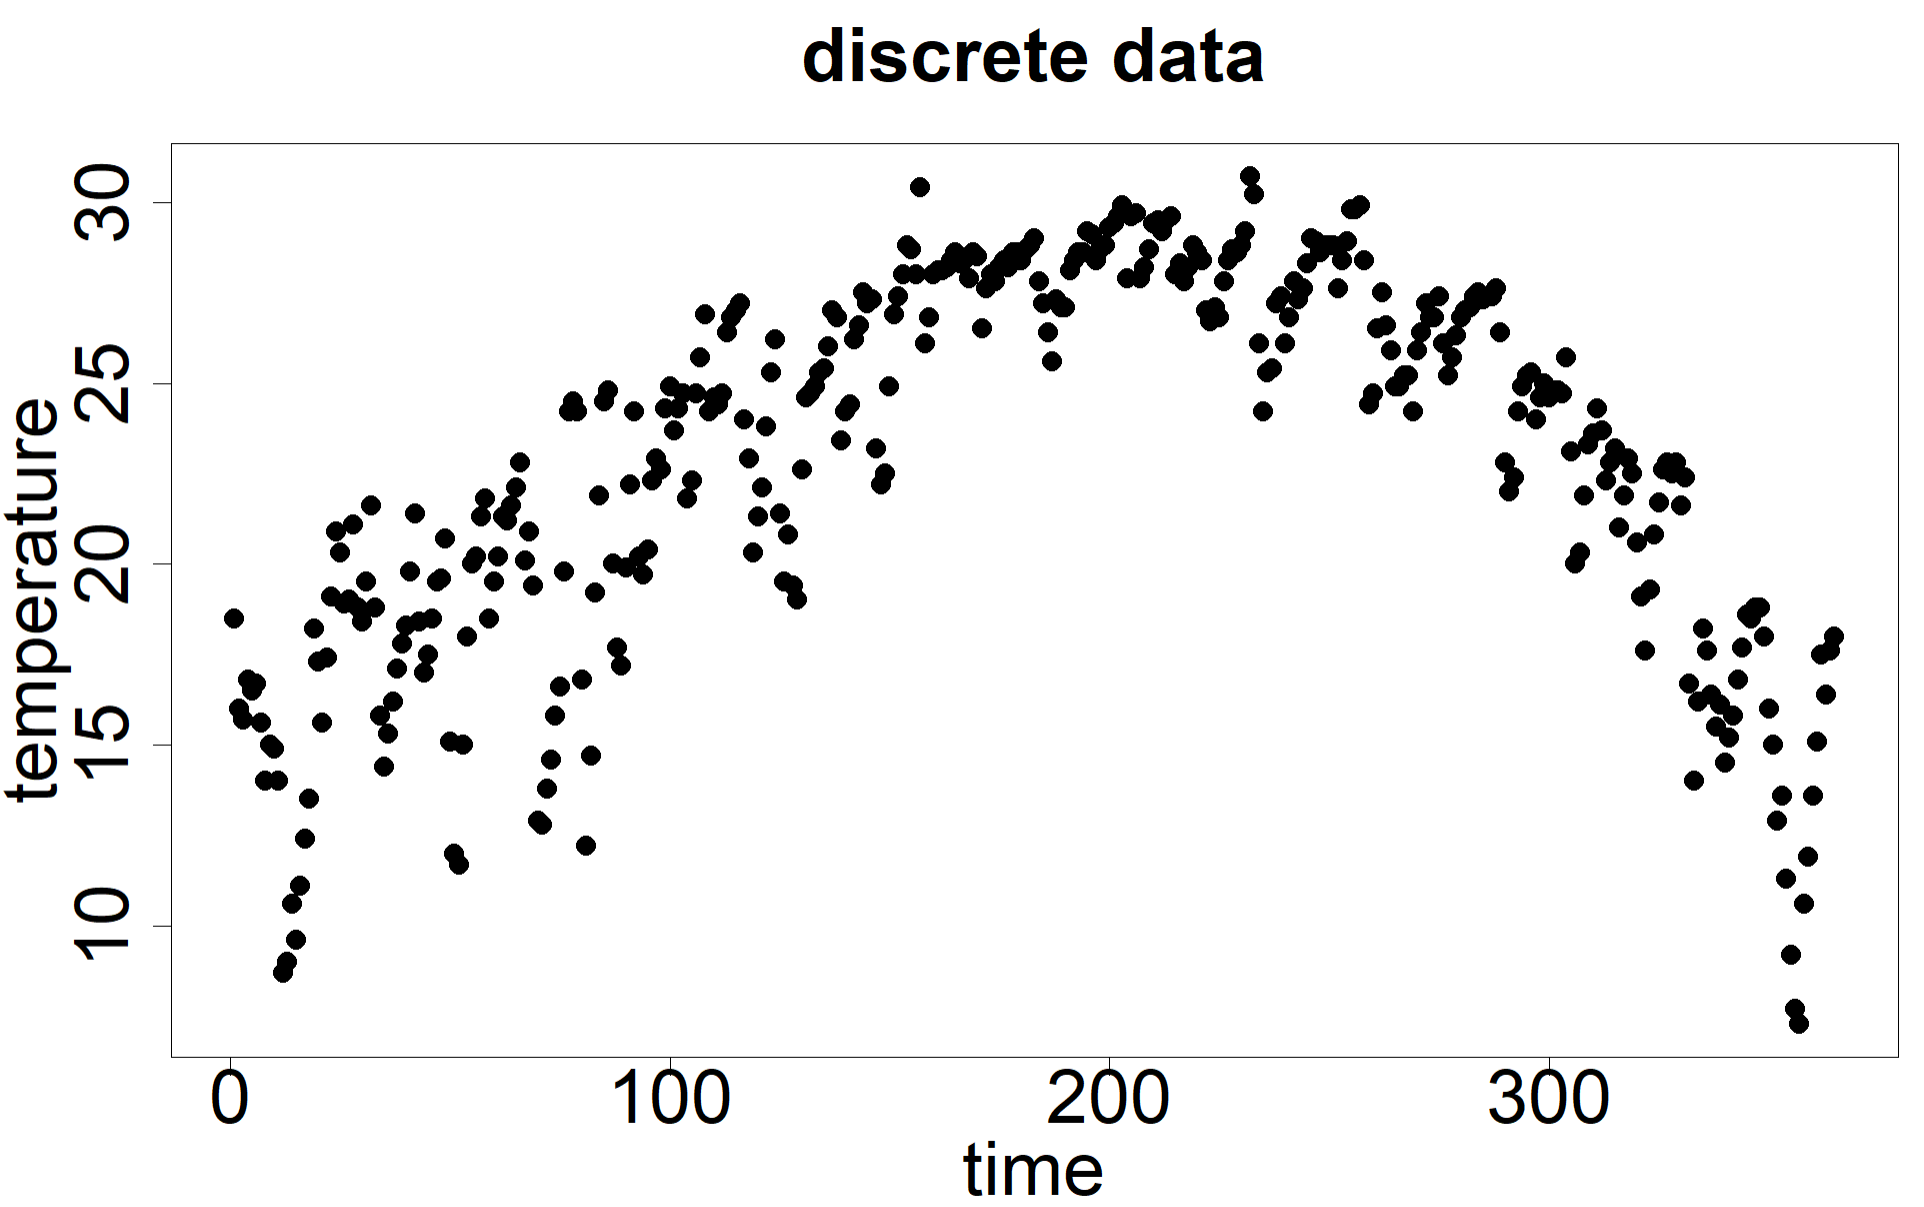
\includegraphics[width=0.47\textwidth]{temp example1}}
	\subfigure[]{
	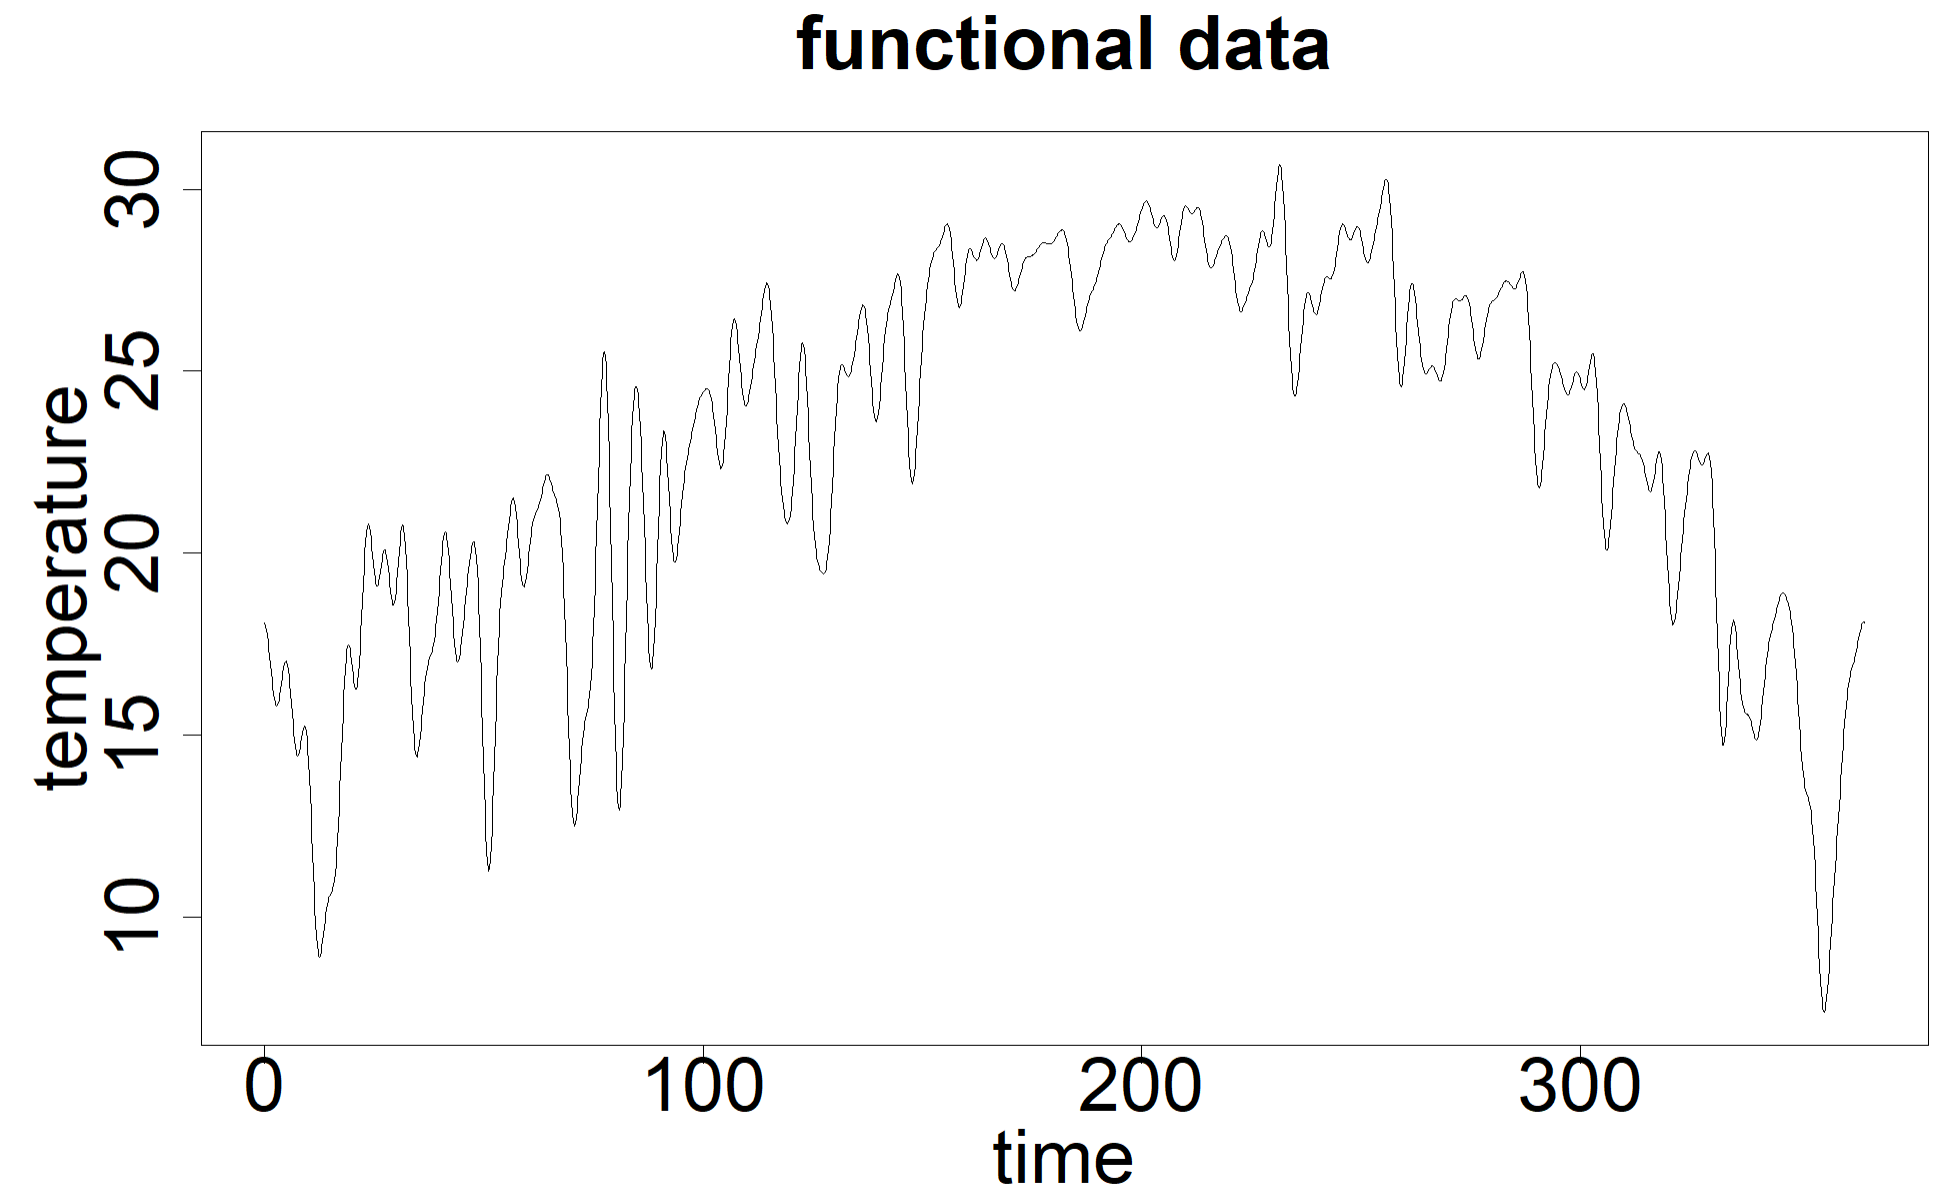
\includegraphics[width=0.47\textwidth]{temp example2}}
	\caption{The daily average temperature in Macau (1999) }
	\end{figure}

	\bigskip % Vertical whitespace
	
	
	\bigskip % Vertical whitespace
	
\end{frame}


%------------------------------------------------

\subsection{Smooth}

\begin{frame}
	\frametitle{Basis and estimation}
	Basis function expansion: 
	$$x(t) = \sum_{k=1}^Kc_k\phi_k(t) = \bm{c}'\bm{\phi}(t)$$
	Type of basis function systems: constant basis, monomial basis, splines and Fourier series. The Fourier series are:
%	The Fourier basis functions are shown as follows: 
	\begin{align*}
%	\text{Fourier series: \qquad}
	\phi_{1}(t) &= 1\\
	\phi_{2}(t) &= \sin(\omega t)\\
	\phi_{3}(t) &= \cos(\omega t)\\
	\phi_{4}(t) &= \sin(2\omega t)\\
	\phi_{5}(t) &= \cos(2\omega t)\\
	&\quad  \vdots\\
	wher&e \quad \omega = 2 \pi / T.
	\end{align*}
	\end{frame}

%%------------------------------------------------
\begin{frame}
	\frametitle{Basis and estimation}
	The loss function for coefficients: 
\begin{align*}
	F(\bm c) &= \sum_j [y_j -x(t_j) ]^2 + \lambda\int [Lx(t)]^2 dt\\
               &= \sum_j [y_j - \bm{c}'\bm{\phi}(t_j)]^2 + \lambda \bm c'(\int [L\bm{\phi}(t) L\bm{\phi}'(t)] dt)  \bm c
\end{align*}
	where $L$ (linear differential operator): a linear combination of derivatives like $Lx = D^2 x$ and harmonic accelerarion $L = \omega^2 D + D^3$.\\	
	\bigskip
	The coefficients of smoothing can be estimated by least square method:  
	\[\hat{\bm c} = (\bm{\Phi}'\bm{\Phi} +\lambda R)^{-1}\bm{\Phi}'y,\]
	where $$R = \int L\bm{\phi}(t)L\bm{\phi}'(t)\mathrm{d}t.$$
	\end{frame}

%%------------------------------------------------


\subsection{Functional linear model}

\begin{frame}
	\frametitle{Functional linear model}
	\begin{itemize}
	\item Comparison: \\
	Traditional LM: $y_i=\ \sum_{j=0}^{p}\beta_j{x_{ij}}+\epsilon_i.$
	\\	
	Functional LM: $y_i=\alpha_0+\bm{z}_{i}^\prime\bm{\alpha}+ \sum_{j=1}^{q}\int\beta_j(t){x_{ij}\left(t\right)dt}+\epsilon_i$.
	\bigskip
	\item Expansion of functional coefficients:
	$$\beta\left(t\right)=\ \sum_{k}^{K}{c_k\phi_k\left(t\right)}=\bm{c}^\prime\bm{\phi}\left(t\right).$$	
	
	\end{itemize}
	\end{frame}
%------------------------------------------------
\begin{frame}
	\frametitle{Functional linear model}
	\begin{itemize}
	\item Loss function:
	\begin{align*}
	SSE\left(\alpha,\beta\right)&=\sum_{i=1}^N\left[y_i-\bm{z}_{i}^\prime\bm{\alpha}-\sum_{j=1}^{q}\int x_{ij}\left(t\right)\beta_j\left(t\right)dt\right]^2\\
	&=\ \sum_{i=1}^{N}\left[y_i-\bm{z}_{i}^\prime\bm{\alpha}-\sum_{j=1}^{q}c_{ij}\int x_{ij}\left(t\right)\phi_j\left(t\right)dt\right]^2
	\end{align*}
	\\	
	\begin{align*}
	{\rm PENSSE}_\lambda\left(\bm \alpha,\bm \beta\right)=
	&\sum_{i=1}^N\left[y_i-z_i'\alpha-\sum_{j}\int{x_{ij}\left(t\right)\beta_j\left(t\right)dt}\right]^2\\
	&+\lambda\left(\int{\left[L \bm \beta'\left(t\right) L\bm \beta (t) \right]dt}\right).
	\end{align*}

	\end{itemize}
	\end{frame}
%------------------------------------------------
\begin{frame}
	\frametitle{Functional linear model}
	\begin{itemize}
	\item Matrix form:
	$$\mathbf{Z}=\left[\begin{matrix}\mathbf{z}_\mathbf{1}^\prime&\int{x_{11}\left(t\right)\bm{\Phi}_{1}\left(t\right)dt}\ \ \ \ \ \ldots&\int{x_{1q}\left(t\right)\bm{\Phi}_{q}\left(t\right)dt}\\\vdots&\ddots\ &\vdots\\\mathbf{z}_\mathbf{n}^\prime&\int{x_{n1}\left(t\right)\bm{\Phi}_{1}\left(t\right)dt\ }\ \ \ \ \ldots&\int{x_{nq}\left(t\right)\bm{\Phi}_{q}\left(t\right)dt}\\\end{matrix}\right],$$
	$$\bm{b}=\left[\begin{matrix}\bm{\alpha}\\\bm{c}\\\end{matrix}\right]$$
	$$\bm{y}=\bm{Zb}+\bm{\epsilon}$$
	\item Estimation of coefficient:
	$$\hat{\bm{b}}=\left(\bm{Z}'\bm{Z}\right)^{-{1}}\bm{Z}'\bm{y}$$
	$$\hat{\bm{b}}={\left(\bm{Z}^\prime\bm{Z}+\bm{R}(\bm{\lambda}\right))}^{-{1}}\bm{Z}^\prime\bm{y}$$

	\end{itemize}
	\end{frame}
%------------------------------------------------
\subsection{Functional Principal Component Analysis}
\begin{frame}
\frametitle{Functional Principal Component Analysis}
\begin{table}[!htbp]
\centering
\begin{tabular}{cccccc}
   \toprule
   &Multivariate PCA & Functional PCA \\
   \midrule
   Maximization& $Var(a^T X)$ & $ Var(\int{\xi\left(t\right)X_i\left(t\right)dt})$ \\
\\
   Subjection1 & $||\bm a|| = 1$ & $\int\xi(t)^2\mathrm{d}t = 1$ \\
\\
   Subjection2 & $\bm a_j^T \bm a_k = 0,k<j$ & $\int\xi_j(t)\xi_k(t)\mathrm{d}t = 0,k<j $\\
\\
   Eigenvalue/Eigenvector & $\Sigma \bm a_j = \mu_j \bm a_j$ & $\int v(s,t)\xi_j(t) dt = \mu_j \xi_j(s)$\\
\\

   Score & $c_{ij}=a_j^T x_i$  & $ c_{ij}=\int{\xi_j\left(t\right)x_i\left(t\right)dt}$\\
\\
   FVE& $\frac{\sum_{j=1}^q \mu_j}{\sum \mu_j}$  & $\frac{\sum_{j=1}^q \mu_j}{\sum \mu_j}$\\
   \bottomrule
\end{tabular}
\caption{Comparison between multivariate PCA and functional PCA}
\end{table}
Note: $v(s,t) = \frac{1}{N-1}\sum_{i}[x_i(s) - \bar x(s)][x_i(t)-\bar x(t)]$
\end{frame}
%------------------------------------------------
\subsection{Functional Score Regression}
\begin{frame}
\frametitle{Functional Score Regression}
Multivariate PCA: dimension reduction among different variables.\\
\smallskip
Functional PCA: dimension reducntion within one variable.
\bigskip


Functional Score Regression: combination of multivariate PCA and Functional Linear Model
\begin{enumerate}
\item PCA in multivariate data perspective.
\item Smooth their principal component scores and get functional score.
\item Replace functional scores to original functional variables in the FLM.
\end{enumerate}

\end{frame}
%------------------------------------------------

\section{Functional Deep Learning}
\begin{frame}
	\frametitle{Artificial Neural Network}
	Without taking functional data into consideration
	\begin{columns}[t]
		\begin{column}{0.5\textwidth}
			\begin{figure}
				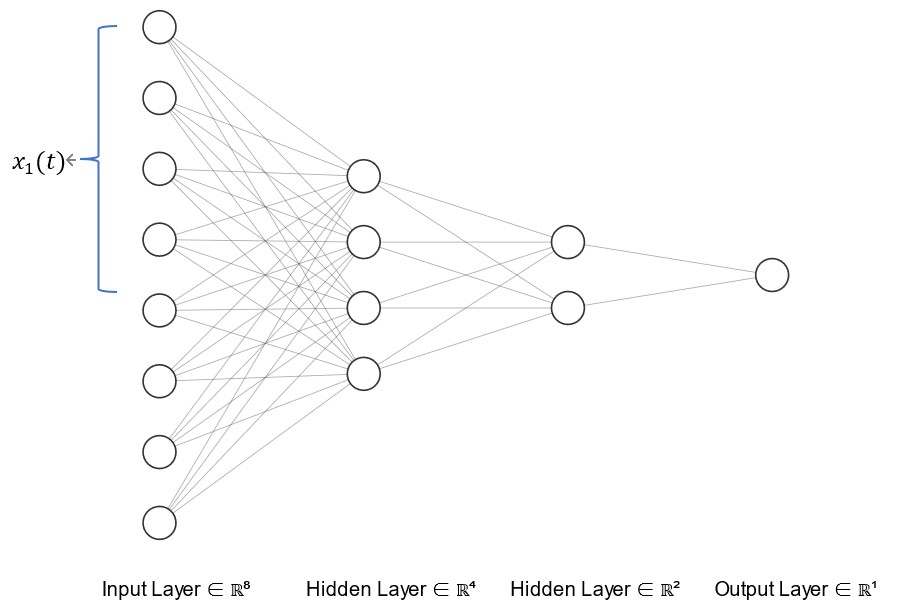
\includegraphics[width=0.9\linewidth]{fnn1.jpg}
				\caption{ANN}
			\end{figure}
		\end{column}
		\begin{column}{0.5\textwidth}
			\begin{itemize}
			\item Advantage:\\
			Easy to understand and implement
			\bigskip
			\item Disadvantage:\\
			\begin{enumerate}
			\item Too many parameters.
			\smallskip
%			\item Sensitive to outliers.
%			\smallskip
			\item Lack of interpretation for weight function.
			\end{enumerate}		
			\end{itemize}
		\end{column}
	\end{columns}
\end{frame}
%------------------------------------------------
\subsection{Functional Neural Network}
\begin{frame}
	\frametitle{Functional Neural Network}
	\begin{figure}
	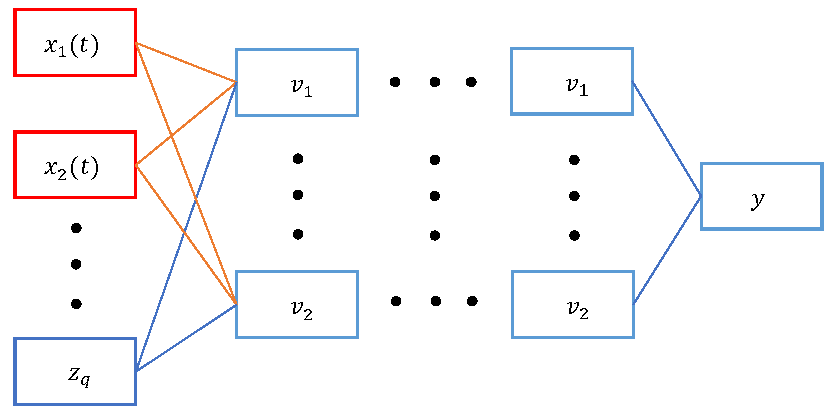
\includegraphics[width=0.73\linewidth]{fnn4.pdf}
	\caption{FuncNN}
	\end{figure}
	Introduce functional data into neural network accroding to FuncNN (Thind et al. ,2022). They do some manipulations in the first layer of network and then follow the same rules of traditional network. Formulate neuron $v$ as:
	$$v_i^{(1)} = g\Big(\sum_{k=1}^K \int_\mathcal{T}\beta_{ik}(t)x_k(t)\mathrm{d}t + \sum_{j=1}^Jw_{ij}^{(1)}z_j + b_i^{(1)}\Big)$$
		
\end{frame}
%------------------------------------------------

\begin{frame}
	\frametitle{Functional Neural Network}
	Details about the first layer and weight function are shown in graph: 	
	\begin{figure}
	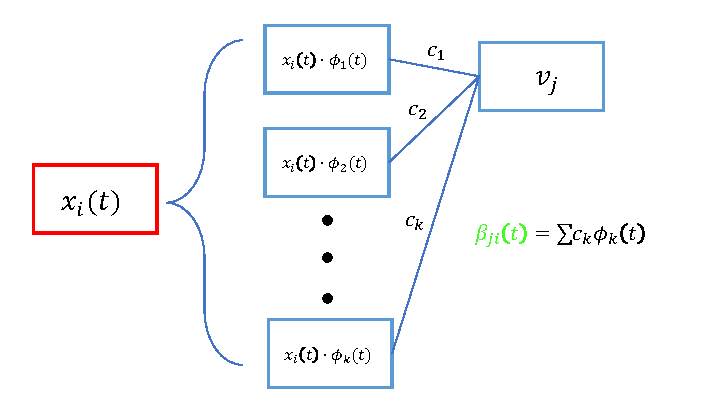
\includegraphics[width=0.5\linewidth]{fnn5.pdf}
%	\caption{FuncNN}
	\end{figure}
	Weight function can be expressed by basis function expansion: 
	$$\beta_{ji}(t) = \sum_{k=1}^{K} c_{ijk}\phi_{ijk}(t)$$
	Then neuron $v$ is formulated as:
	\[v_i^{(1)} = g\Big(\sum_{j=1}^J \sum_{k=1}^{K}\int_\mathcal{T}\phi_{ijk}(t)x_j(t)\mathrm{d}t + \sum_{p=1}^Pw_{ip}^{(1)}z_p + b_i^{(1)}\Big)\]		
\end{frame}
%------------------------------------------------
\section{Data}

\begin{frame}
	\frametitle{Data description}	
	\begin{itemize}
	\item Source: Macau Meteorological and Geophysical Bureau
	\bigskip
	\item Data details: daily average temperature, daily average relative humidity, daily average wind speed, daily average sea level pressure, daily total sunshine duration, and daily average precipitation
	\bigskip
	\item Variable: response and covariates
		\begin{itemize}
		\item Scalar Response: precipitation
		\item Functional Covariates: temperature, humidity, pressure, sunshine, windspeed
		\end{itemize}
	\bigskip
	\item Time interval: 1999.01.01-2022.12.31.\\
		24 years as 24 functional observations with 365 time points.\\
		5 functional covarites and 1 scalar response.
	\end{itemize}
\end{frame}
%------------------------------------------------
\section{Result}
\subsection{Smooth}
\begin{frame}
	\frametitle{Choosing number of basis functions}	
	We choose Fourier Series as bases and the number of basis funtions is determined by AIC + BIC, take covariate temperature as example: 
	\begin{figure}[H]
	\centering  %图片全局居中
	\subfigure[]{
	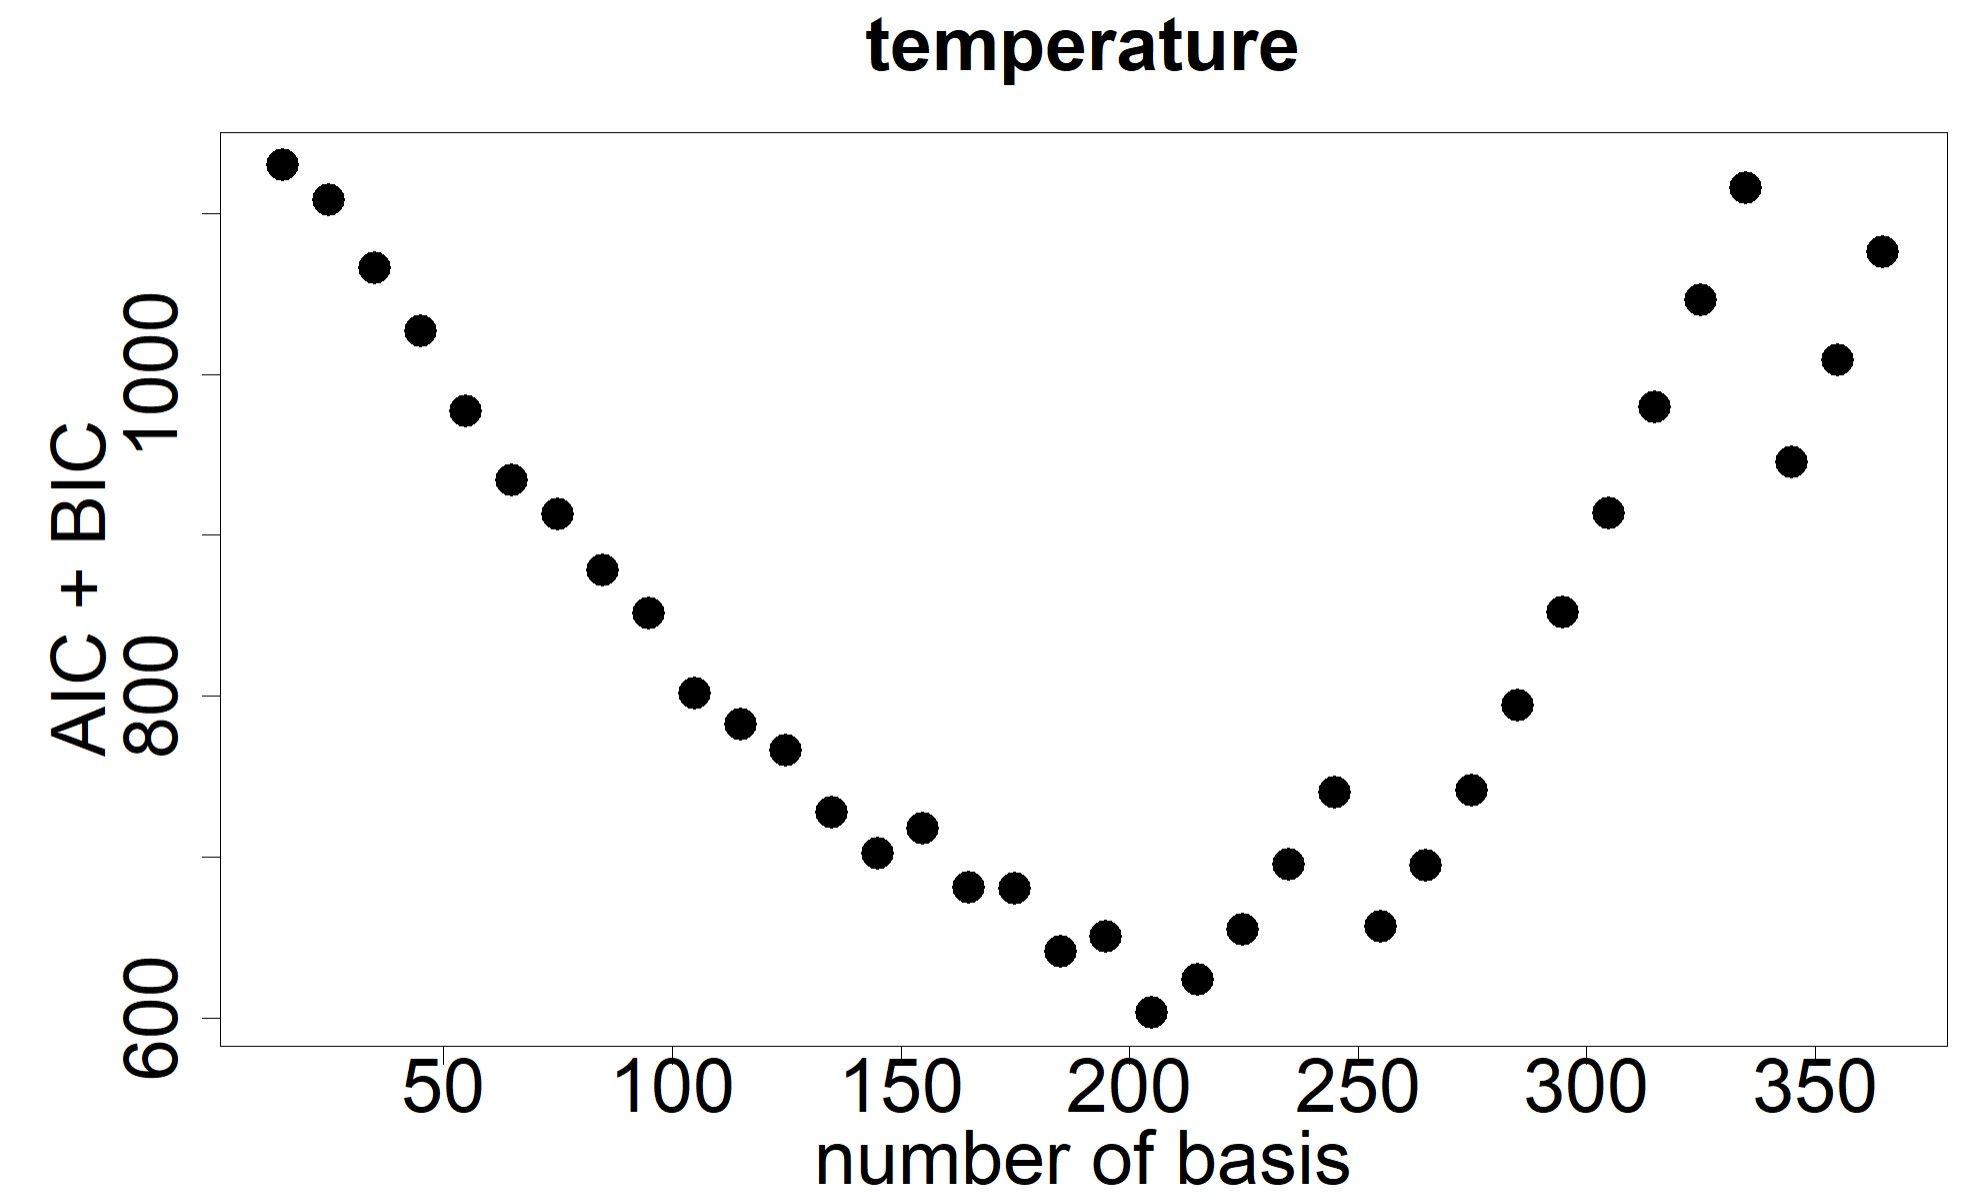
\includegraphics[width=0.47\textwidth]{temp1}}
	\subfigure[]{
	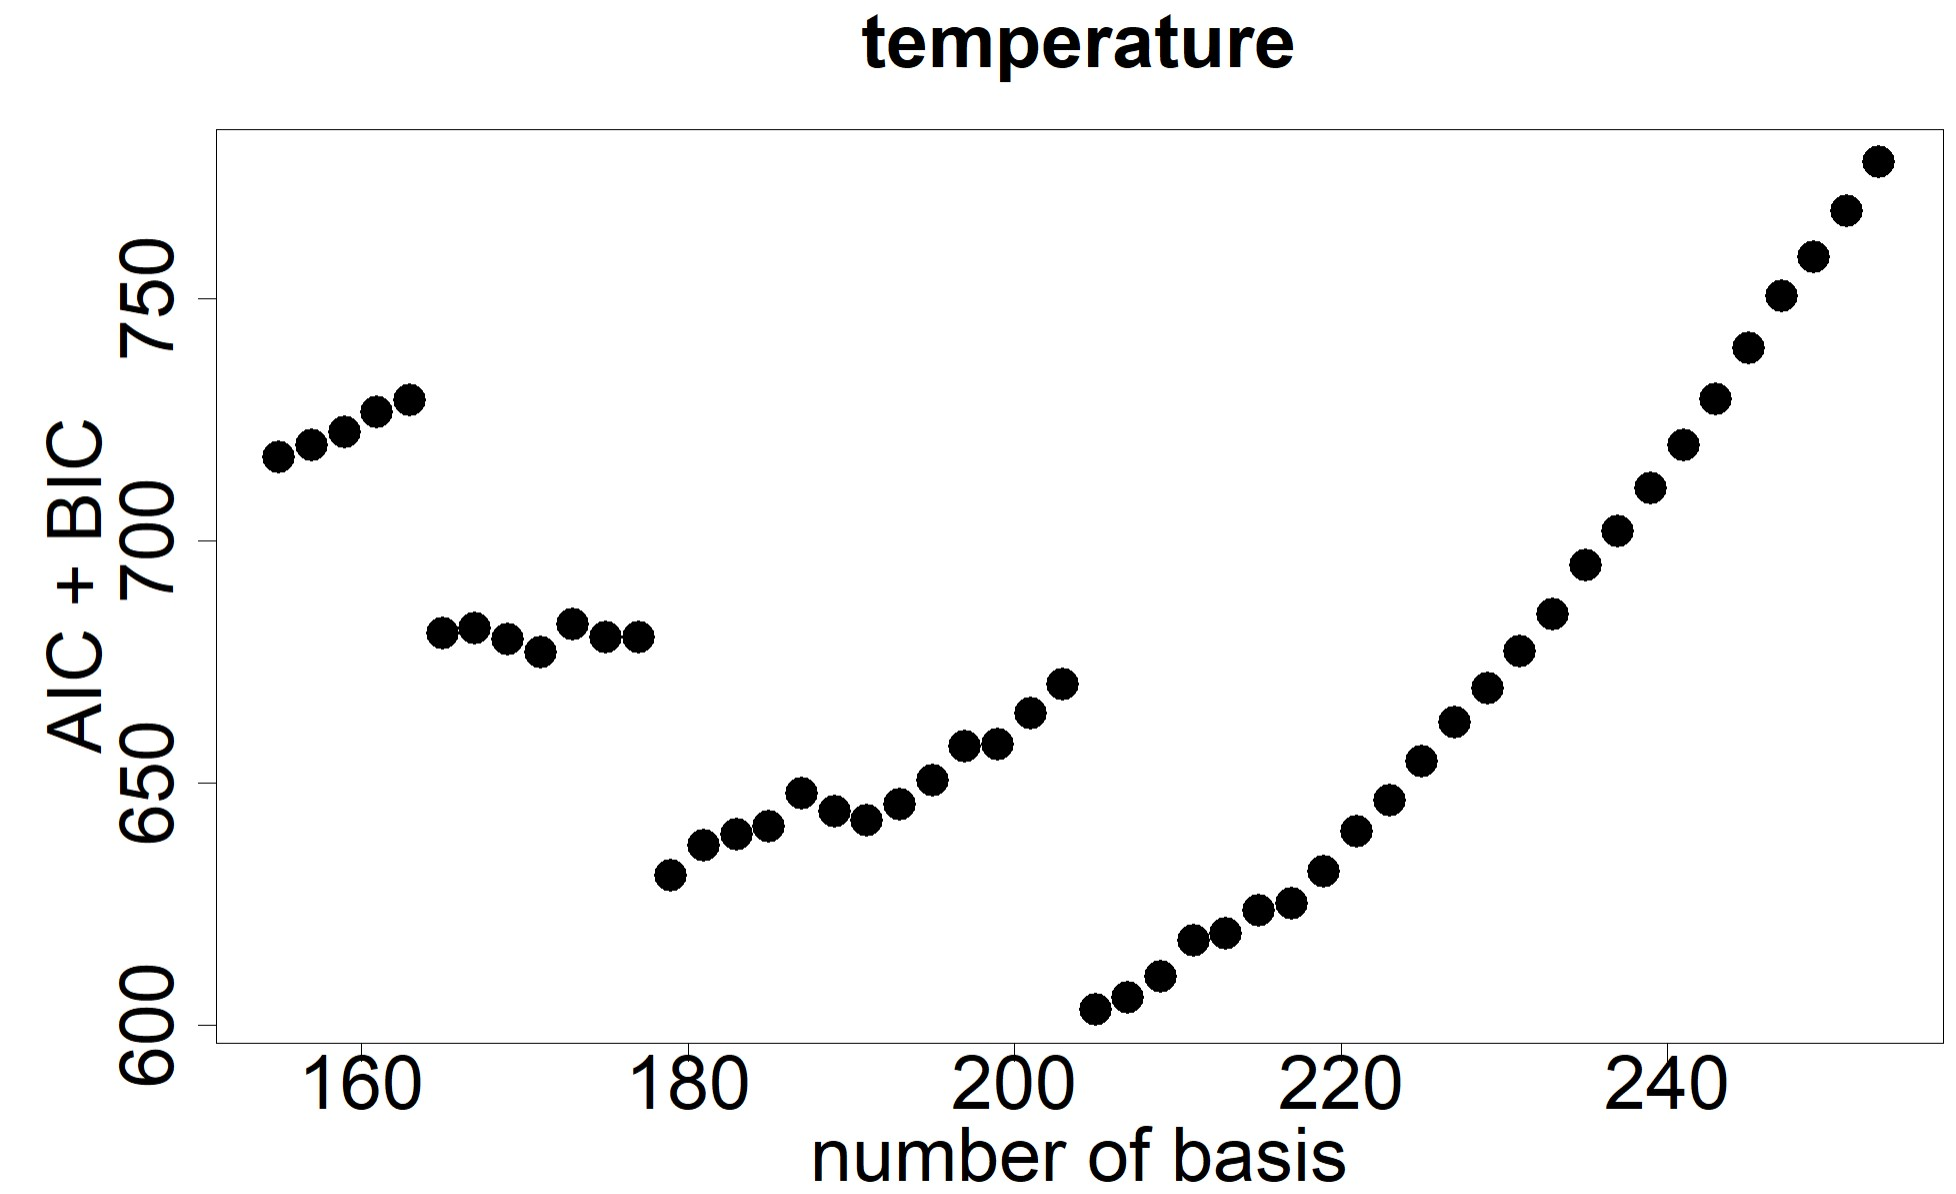
\includegraphics[width=0.47\textwidth]{temp2}}
	\caption{The value of AIC + BIC corresponding to each $log_{10}(\lambda)$ for Temperature}
	\end{figure}
\end{frame}

%------------------------------------------------
\subsection{Model Building}
\begin{frame}
	\frametitle{Functional Linear Model (FLM)}
	After we smooth the data, we plug in functional data obtained into 4 models discussed before, implememnt the models with more details.
	\bigskip \\
	For functional linear model:
	\begin{itemize}
	\item Due to sample size, we can only take 3 basis functions for each covariate, otherwise $Z'Z$ is a singular matrix, i.e. not invertible. And the results is terrible.
	\bigskip
	\item So it is necessary to add a penalty term, then $Z'Z+R(\lambda)$ is invertible for more than 3 basis functions.
	\end{itemize}
\end{frame}
%------------------------------------------------
\begin{frame}
	\frametitle{Functional Score Regression (FSR)}
	We take PCA of five covariates in 24 years and the total variance explained by different PCs are shown in picture.
	\begin{figure}
	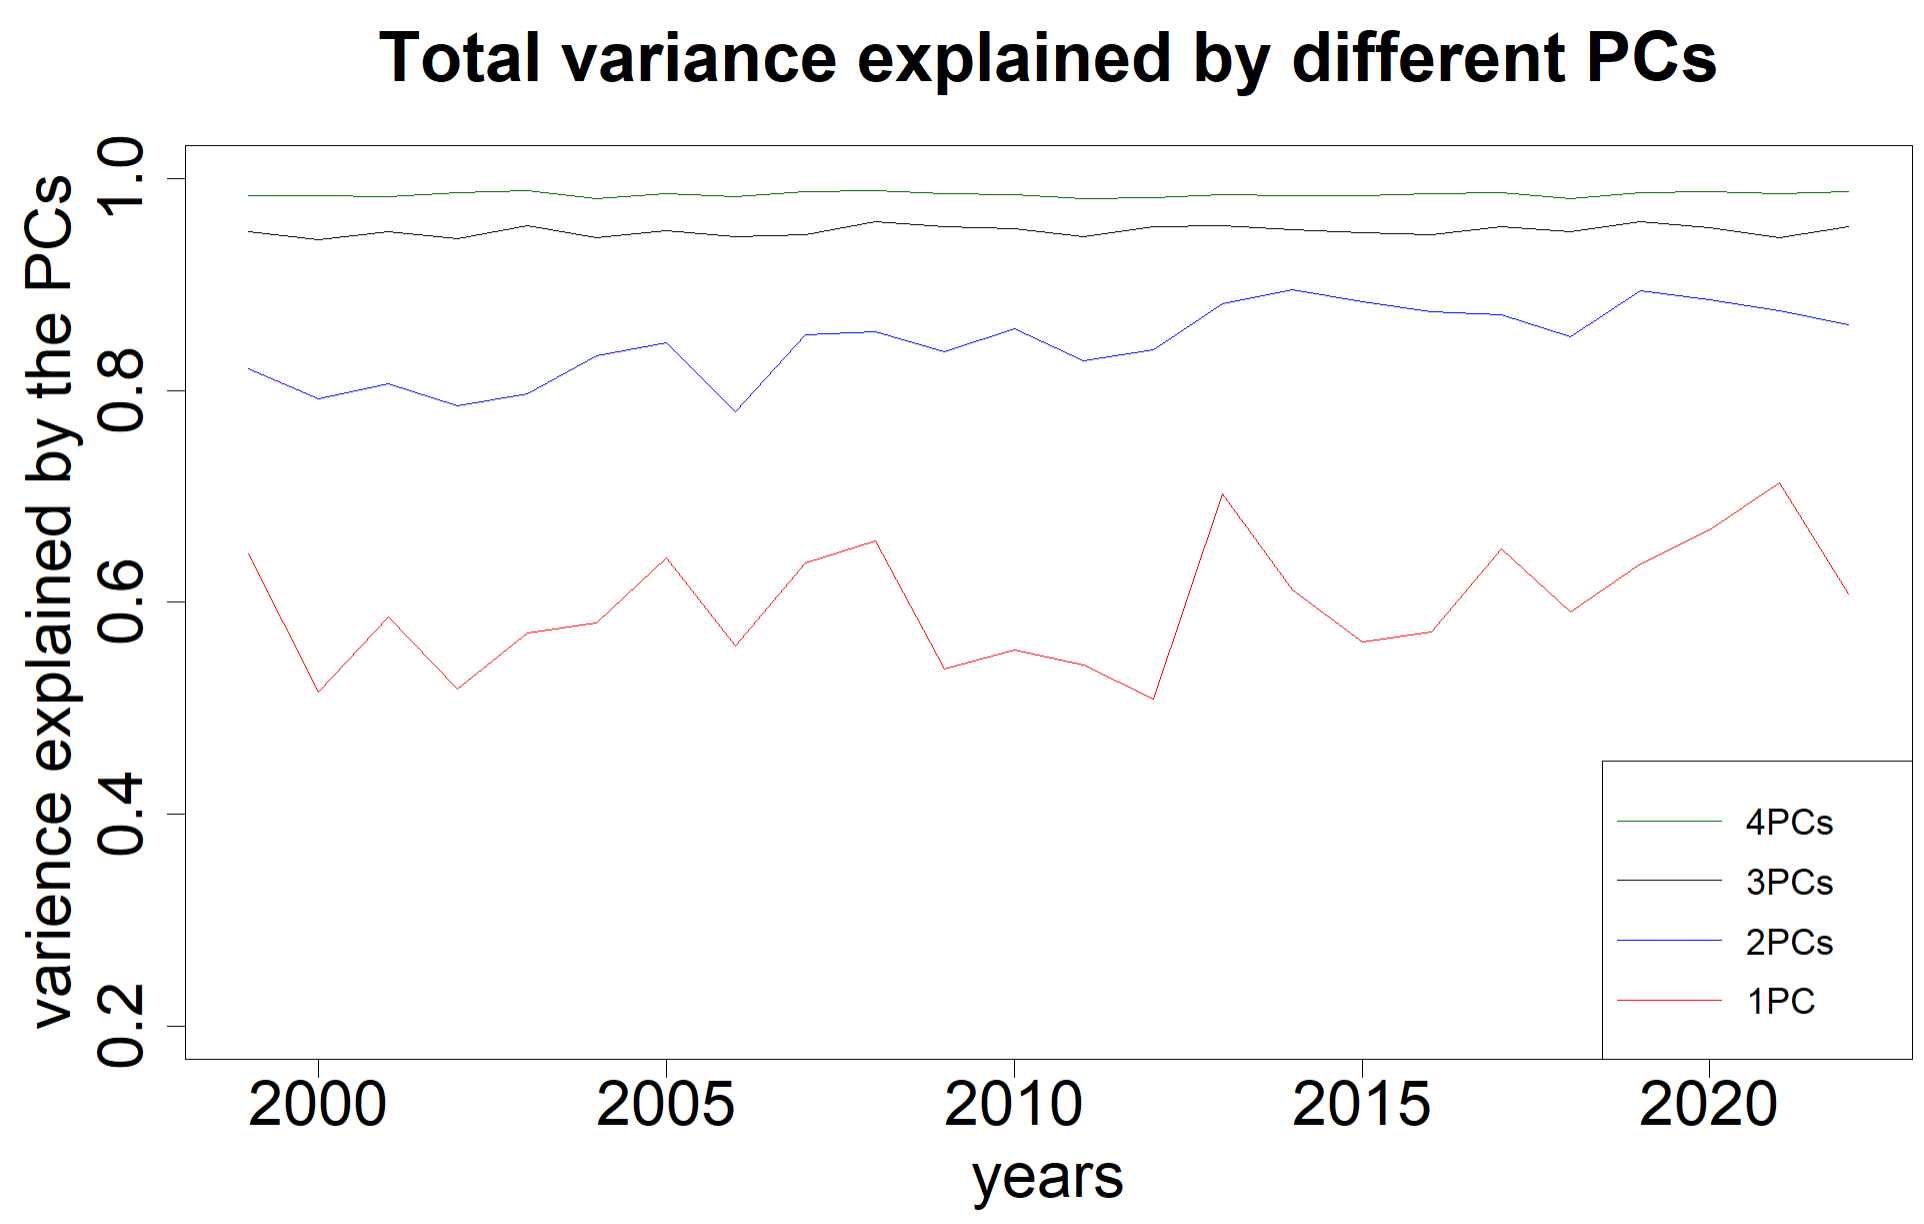
\includegraphics[width=0.65\linewidth]{3PCs.png}
	\caption{FVE of PCs}
	\end{figure}
	We choose the first three functional scores as our covariates.
\end{frame}
%------------------------------------------------
\begin{frame}
	\frametitle{Functional Neural Network (FuncNN)}
	Hyperparameters of FuncNN
	\begin{itemize}
	\item number of layers 
	\item number of neurons per layer 
	\item activation function: ReLU, sigmoid, linear, LeakyReLU, tanh
	\item method to avoid overfitting: dropout and early stop
	\end{itemize}
\end{frame}
%------------------------------------------------
\subsection{Model measurement}
\begin{frame}
	\frametitle{Measurement techniques}
	Techniqes we use to measure the models: 
	\begin{itemize}
	\item Training set and test set split
	\bigskip
	\item $MSPE_{CV}=\ \sum_{b=1}^{B}\sum_{l\in S_b}^{N}{\frac{\left({\hat{y}}^{\left(-b\right)}-y_l\right)^2}{N}\ }$, $S_b$ is the $b$-th partition of the training data set and $\hat{y}^{(-b)},l \in S_b$ is the prediction in the set. Here we set $b$ as 5, namely we use five-fold cross-validation.
	\bigskip
	\item $R^2=1-\ \sum_{l=1}^{N}{\left(y_l-{\hat{y}}_l\right)^2/\sum_{l=1}^{N}\left(y_l-\bar{y}\right)^2}.$
	\end{itemize}
\end{frame}
%------------------------------------------------
\begin{frame}
\frametitle{Outcomes of different models}
For the current year regression problem:
\numberwithin{table}{section}
\begin{table}[!htbp]
\centering
\begin{tabular}{cccccc}
   \toprule
   &$Training \quad MSE$ & $MSPE_{cv}$ & $Test\quad MSE$ & $Test\quad R^2$ \\
   \midrule
   FLM without penalty&0.20&---&4.07&-1.83 \\
   FLM with penalty&1.02&1.92&1.43&0.003 \\
   FSR& 0.65&1.28&0.95&0.34\\
   FuncNN&0.33&1.50&0.70&0.51\\
   \bottomrule
\end{tabular}
\caption{Result for the current year regression problem}
\end{table}

For the next year's prediction problem (autoregression):


\numberwithin{table}{section}
\begin{table}[!htbp]
\centering
\begin{tabular}{cccccc}
   \toprule
   &$Training\quad MSE$ & $MSPE_{cv}$ & $Test\quad MSE$ & $Test\quad R^2$ \\
   \midrule
   FLM without penalty&---&---&---&--- \\
   FLM with penalty&1.09&0.89&1.73&-0.20\\
   FSR& 1.02&1.32&1.28&0.11\\
   FuncNN&0.79 &1.48 &1.05 &0.27\\
   \bottomrule
\end{tabular}
\caption{Result for the next year prediction problem}
\end{table}
\end{frame}
%------------------------------------------------
\section{Discussion}
\begin{frame}
	\frametitle{Conclusion and further work}
	\begin{itemize}
	\item Conclusion: FuncNN performs well and the reason may be the relation between response and covariates is not linear 
	\bigskip
	\item Further work:
	\smallskip
		\begin{itemize}
		\item Few criteria to decide number of basis functions in the process of smoothing
		\smallskip
		\item Few methods to deal with the problem of multicollinearity
		\smallskip
		\item Few formal significance test of functional coefficients
		\smallskip
		\item FuncNN deals with functional data only in the first layer.
		\end{itemize}
	\end{itemize}
\end{frame}





%------------------------------------------------

\section{Reference}

%\begin{frame}
%	\frametitle{Citing References}
%	
%	An example of the \texttt{\textbackslash cite} command to cite within the presentation:
%	
%	\bigskip % Vertical whitespace
%	
%	This statement requires citation \cite{p1,p2}.
%\end{frame}

%------------------------------------------------

\begin{frame}% Use [allowframebreaks] to allow automatic splitting across slides if the content is too long
	\frametitle{References}
%	
%	\begin{thebibliography}{99} % Beamer does not support BibTeX so references must be inserted manually as below, you may need to use multiple columns and/or reduce the font size further if you have many references
%		\footnotesize % Reduce the font size in the bibliography
%		
%		\bibitem[Smith, 2022]{p1}
%			John Smith (2022)
%			\newblock Publication title
%			\newblock \emph{Journal Name} 12(3), 45 -- 678.
%			
%		\bibitem[Kennedy, 2023]{p2}
%			Annabelle Kennedy (2023)
%			\newblock Publication title
%			\newblock \emph{Journal Name} 12(3), 45 -- 678.
%	\end{thebibliography}
\tiny{
\begin{enumerate}
\item Cuesta-Albertos, J. A., García-Portugués, E., Febrero-Bande, M., \& González-Manteiga, W. (2019). Goodness-of-fit tests for the functional linear model based on randomly projected empirical processes. The Annals of Statistics, 47(1), 439-467.
\item Ferraty F, Vieu P (2006). Nonparametric Functional Data Analysis. Springer-Verlag, New York.  
\item Heinrichs, F., Heim, M., \& Weber, C. (2023). Functional Neural Networks: Shift invariant models for functional data with applications to EEG classification. arXiv preprint arXiv:2301.05869.
\item Henderson, B. (2006). Exploring between site differences in water quality trends: a functional data analysis approach. Environmetrics: The official journal of the International Environmetrics Society, 17(1), 65-80.
\item Martínez, J., Saavedra, Á., García-Nieto, P. J., Piñeiro, J. I., Iglesias, C., Taboada, J., ...\& Pastor, J. (2014). Air quality parameters outliers detection using functional data analysis in the Langreo urban area (Northern Spain). Applied Mathematics and Computation, 241, 1-10.
\item Perdices, D., de Vergara, J. E. L., \& Ramos, J. (2021). Deep-FDA: Using functional data analysis and neural networks to characterize network services time series. IEEE Transactions on Network and Service Management, 18(1), 986-999.
\item Preda, C., Saporta, G., and Lévéder, C. (2007), “PLS Classification of Functional Data,” Computational Statistics, 22, 223–235.  
\item Ramsay, J. O., Hooker, G., \& Graves, S. (2009). Functional data analysis with R and MATLAB (Vol. 43). Springer Science \& Business Media.
\item Rumelhart, D., Hinton, G., and Williams, R. (1985), “Learning Internal Representations by Error Propagation,” Technical Report, California Univ San Diego La Jolla Inst for Cognitive Science.
\item Srivastava, N., Hinton, G., Krizhevsky, A., Sutskever, I., \& Salakhutdinov, R. (2014). Dropout: a simple way to prevent neural networks from overfitting. The journal of machine learning research, 15(1), 1929-1958.
\item Thind, B., Multani, K., \& Cao, J. (2022). Deep Learning With Functional Inputs. Journal of Computational and Graphical Statistics, 00(0), 1-10. 
\item Wang, J.-L., Chiou, J.-M., \& Muller, H.-G. (2015). Functional data analysis. Annual Review of Statistics and Its Application, 2(1), 1–41. 
\item Yao, J., Mueller, J., \& Wang, J. L. (2021, July). Deep learning for functional data analysis with adaptive basis layers. In International Conference on Machine Learning (pp. 11898-11908). PMLR.
\item Yao, Y., Rosasco, L., \& Caponnetto, A. (2007). On early stopping in gradient descent learning. Constructive Approximation, 26(2), 289-315.
\end{enumerate}}
\end{frame}

%----------------------------------------------------------------------------------------
%	ACKNOWLEDGMENTS SLIDE
%----------------------------------------------------------------------------------------

%\begin{frame}
%	\frametitle{Acknowledgements}
%	
%	\begin{columns}[t] % The "c" option specifies centered vertical alignment while the "t" option is used for top vertical alignment
%		\begin{column}{0.45\textwidth} % Left column width
%			\textbf{Smith Lab}
%			\begin{itemize}
%				\item Alice Smith
%				\item Devon Brown
%			\end{itemize}
%			\textbf{Cook Lab}
%			\begin{itemize}
%				\item Margaret
%				\item Jennifer
%				\item Yuan
%			\end{itemize}
%		\end{column}		
%		\begin{column}{0.5\textwidth} % Right column width
%			\textbf{Funding}
%			\begin{itemize}
%				\item British Royal Navy
%				\item Norwegian Government
%			\end{itemize}
%		\end{column}
%	\end{columns}
%\end{frame}

%----------------------------------------------------------------------------------------
%	CLOSING SLIDE
%----------------------------------------------------------------------------------------

\begin{frame}[plain] % The optional argument 'plain' hides the headline and footline
	\begin{center}
		{\Huge Thanks for Listening}

%		\bigskip\bigskip % Vertical whitespace
		
%		{\LARGE}
	\end{center}
				\begin{figure}
				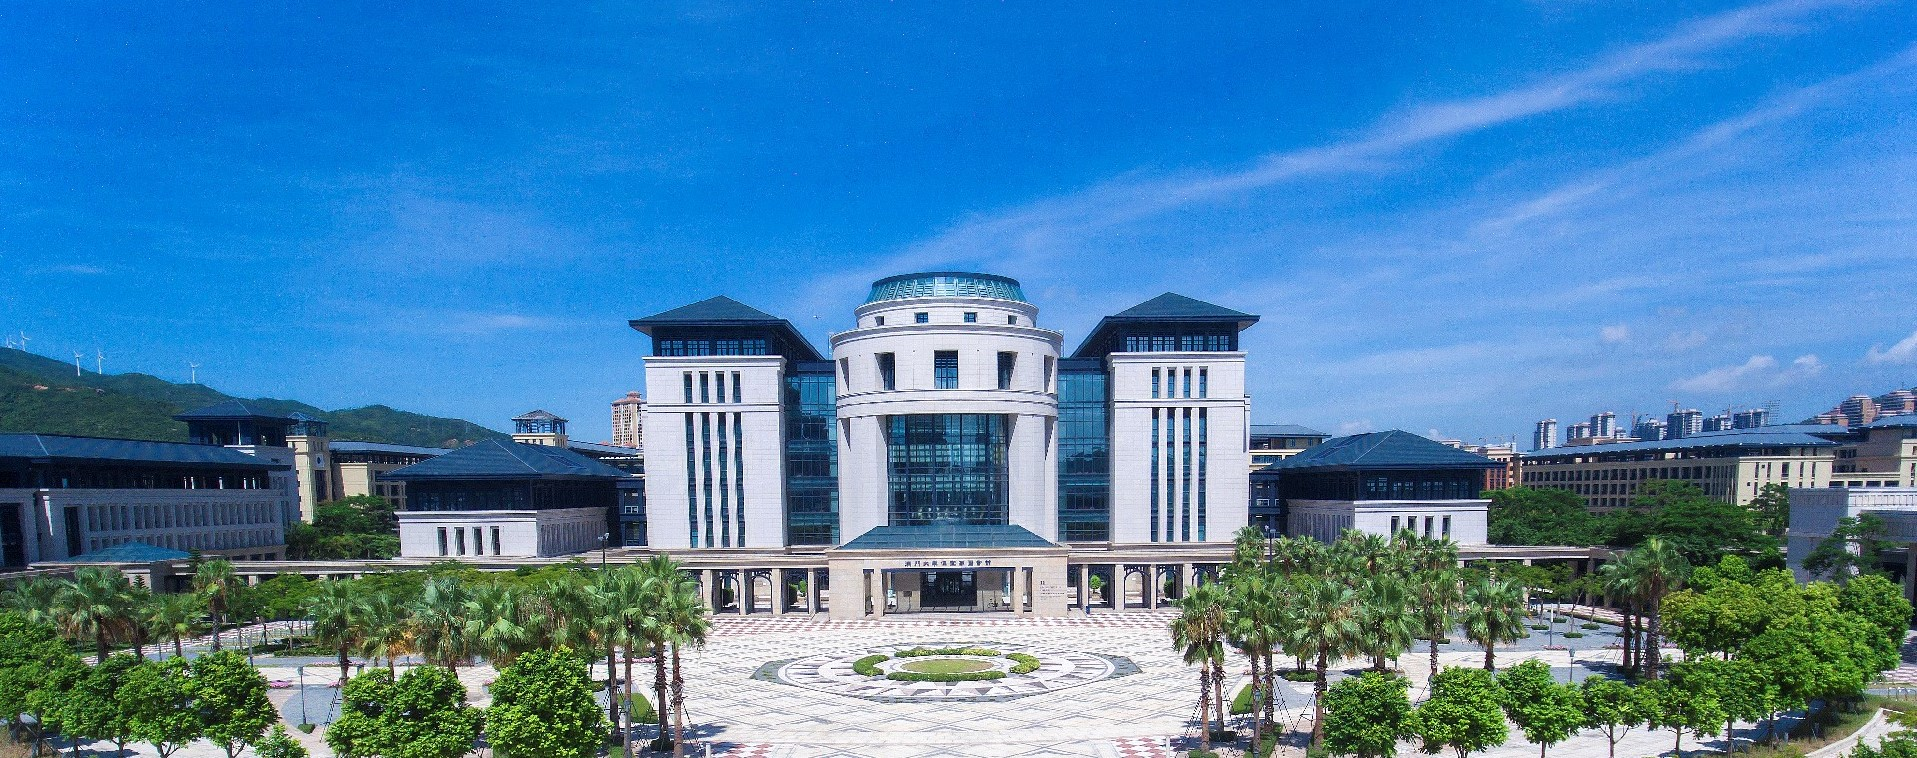
\includegraphics[width=1.0\linewidth]{end.jpg}			
			\end{figure}
		
\end{frame}

%----------------------------------------------------------------------------------------

%------------------------------------------------
\begin{frame}
	\frametitle{Linear Differential Operater}
	$Lx(t)$ is a linear differential operator on $x(t)$. It can be defined as:
	$$
	Lx(t) = \beta_0(t)x(t) + \beta_1(t)Dx(t) +\dots + \beta_{m-1}(t)D_{m-1}x(t) +D_mx(t)
	$$

We choose $L=\omega^2D+D^3$ since we are working on a group of periodical data with a known period, and this penalty can substantially penalize the high-order terms in the Fourier Series. We can see for any periodical data $a_{j}\sin(j\omega t)+b_{j}\cos(j\omega t)$ with known frequency $\omega$, its linear differential operator: 
$$L\left[a_j\sin{\left(j\omega t\right)}+b_j\cos{\left(j\omega t\right)}\right]=\omega^2j\left(1-j^2\right)\left[a_j\cos{\left(j\omega t\right)}-b_j\sin{\left(j\omega t\right)}\right].$$
We observe that when j = 1, there is no penalization. As j increase, the increase of penalty is proportional to $j^2 (1-j^2)^2$ which is very large. Thus, the penalty constricts the form into $a\sin(\omega t) + b\cos(\omega t)$.
	

\end{frame}
%------------------------------------------------
\begin{frame}
	\frametitle{GCV}
	Generalized Cross Validation (GCV):
	$$GCV\left(\lambda\right)=\left(\frac{n}{n-df\left(\lambda\right)}\right)\left(\frac{SSE}{n-df(\lambda)}\right).$$\\
	Let
	$$\bm{R}=\int{L\bm{\phi}\left(t\right)L\bm{\phi}^\prime\left(t\right)dt},$$ 
	If we design the hat matrix as:
	$$\bm{H}=\bm{\Phi}\left(\bm{\Phi}^\prime\bm{\Phi}+\lambda\bm{R}\right)^{-1}\bm{\Phi}^\prime,$$
	then the degree of freedom as a function of $\lambda$ can be calculated by: 
	$$df\left(\lambda\right)=\mathrm{trace}\left[\bm{H}\left(\lambda\right)\right].$$
	Penalty matrix R for functional linear model:
	$$\left[\begin{matrix}\lambda_0 I &\ldots&\ldots&\ldots\\0&\lambda_1R_1&\ldots&0\\\vdots&\vdots&\ddots&\vdots\\0&0&\ldots&\lambda_qR_q\\\end{matrix}\right]$$
\end{frame}
%------------------------------------------------
\begin{frame}
	\frametitle{Functional Response for FLM}
	The functional linear model can also deal with the functional response using a concurrent model that is estimating functional response by the covariates at the same time points. The model can be described as:
	$$\bm{y}(t)=\bm{Z}\left(t\right)\bm{\beta}(t)+\bm{\epsilon}(t),$$
	where $\bm y(t)$ is a functional vector with length $N$ containing $N$ functional response and $\bm Z(t)$ is a functional covariate matrix with dimension $N\times p$. The loss function is similar but only replaces the square term with the inner product on the vector. Then solve the regression by normal equations:
	$$\left[\int{\bm{\Theta}^\prime\left(t\right)\bm{Z}^\prime\left(t\right)\bm{Z}\left(t\right)\bm{\Theta}\left(t\right)dt}+\bm{R}\left(\bm{\lambda}\right)\right]^2\hat{\bm{b}}=\left[\int{\bm{\Theta}^\prime\left(t\right)\bm{Z}^\prime\left(t\right)\bm{y}\left(t\right)dt}\right].$$
	where $\bm\Theta(t)$ is the basis function matrix of functional weight $\bm \beta(t)$, and  $\hat{\bm b}$ is the corresponding coefficient scalar vector.	
	

\end{frame}
%------------------------------------------------
\begin{frame}
	\frametitle{Functional Response for FuncNN}
	FuncNN can also deal with the functional response and its method is quite straightforward if we know how to deal with functional covariates. It still expresses weight functions to functional response as basis functions expansion, takes the inner product of response and basis functions as output neurons, trains the network, and finally output coefficients indicating the weight functions.	

\end{frame}
%------------------------------------------------
\begin{frame}
	\frametitle{Precipitation data}
	\begin{figure}[H] %H为当前位置,!htb为忽略美学标准,htbp为浮动图形
	\centering %图片居中
	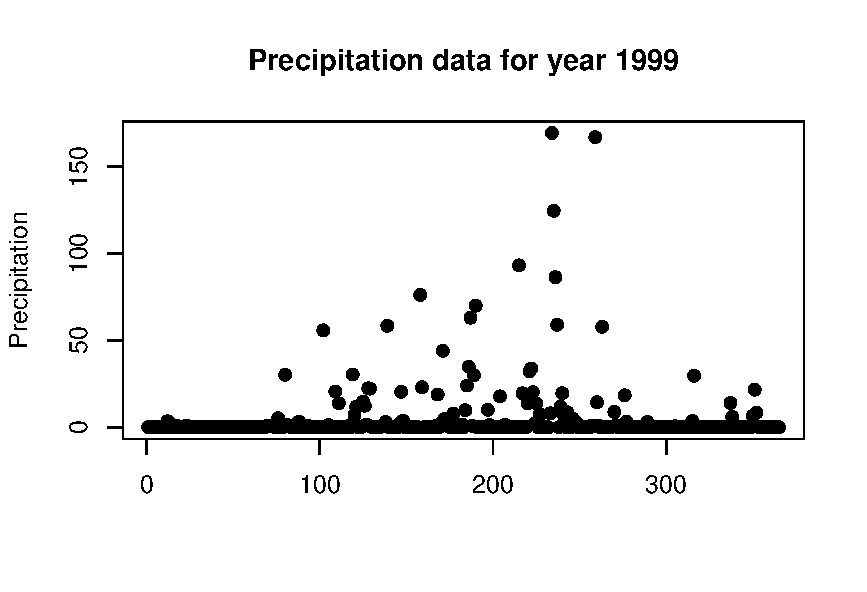
\includegraphics[width=1.0\textwidth]{Prec.pdf} %插入图片,[]中设置图片大小,{}中是图片文件名
	\end{figure}
\end{frame}	
%------------------------------------------------
\begin{frame}
	\frametitle{Precipitation data}
	\begin{figure}[H] %H为当前位置,!htb为忽略美学标准,htbp为浮动图形
	\centering %图片居中
	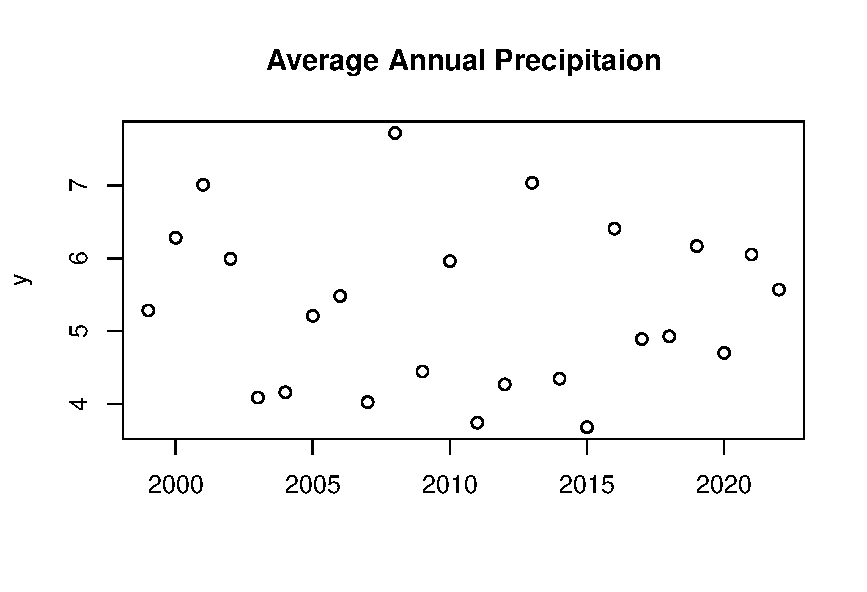
\includegraphics[width=1.0\textwidth]{y_scatter.pdf} %插入图片,[]中设置图片大小,{}中是图片文件名
	\end{figure}
\end{frame}
%------------------------------------------------
\begin{frame}
	\frametitle{Precipitation data}	
	\begin{figure}[H] %H为当前位置,!htb为忽略美学标准,htbp为浮动图形
	\centering %图片居中
	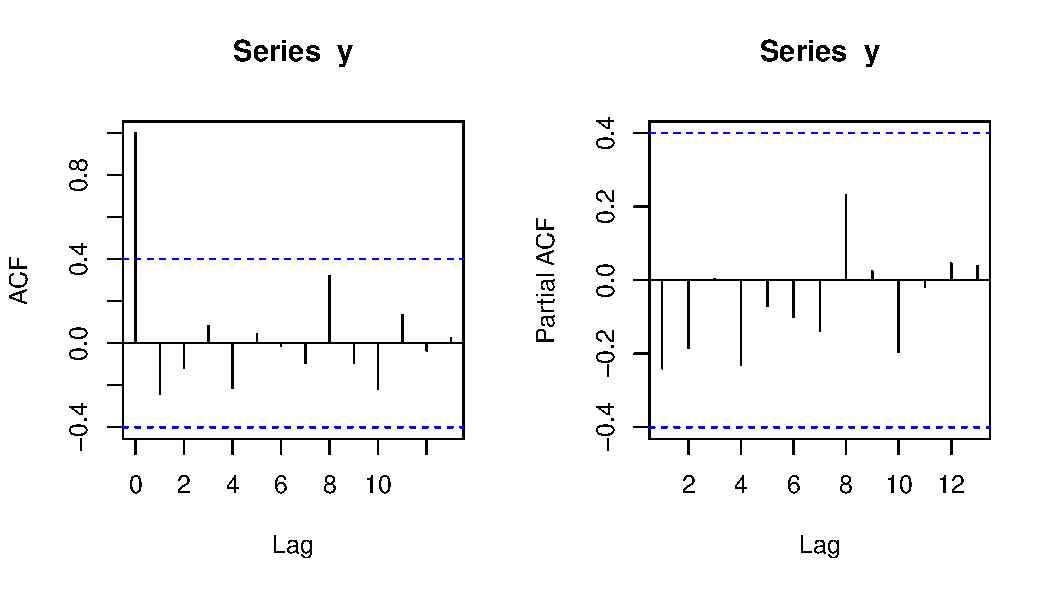
\includegraphics[width=1.0\textwidth]{acf_pacf.pdf} %插入图片,[]中设置图片大小,{}中是图片文件名
	\end{figure}
\end{frame}
%------------------------------------------------
\begin{frame}[allowframebreaks]
	\frametitle{Drop out method}
	Dropout addresses overfitting by randomly "dropping out" (setting to zero) some neurons during training. This forces the network to learn more robust features, as no single neuron can rely on the presence of another neuron to make predictions. During training, each neuron in the network has a probability $p$ of being "dropped out." This means that the neuron's output is set to zero with probability $p$, or left unchanged with probability $1-p$. The value of $p$ is typically set between 0.1 and 0.5.

To implement this method, we generate a Bernoulli distribution with probability $p$ to get a set of (0,1) samples, the number of samples equals to the number of neurons in a hidden layer. If the neuron corresponds to 0, drop it, else remain that neural. The following 2 graphs show how dropout was implemented in a one-hidden layer neural network.
\numberwithin{figure}{section}
\begin{figure}[H] %H为当前位置,!htb为忽略美学标准,htbp为浮动图形
\centering %图片居中
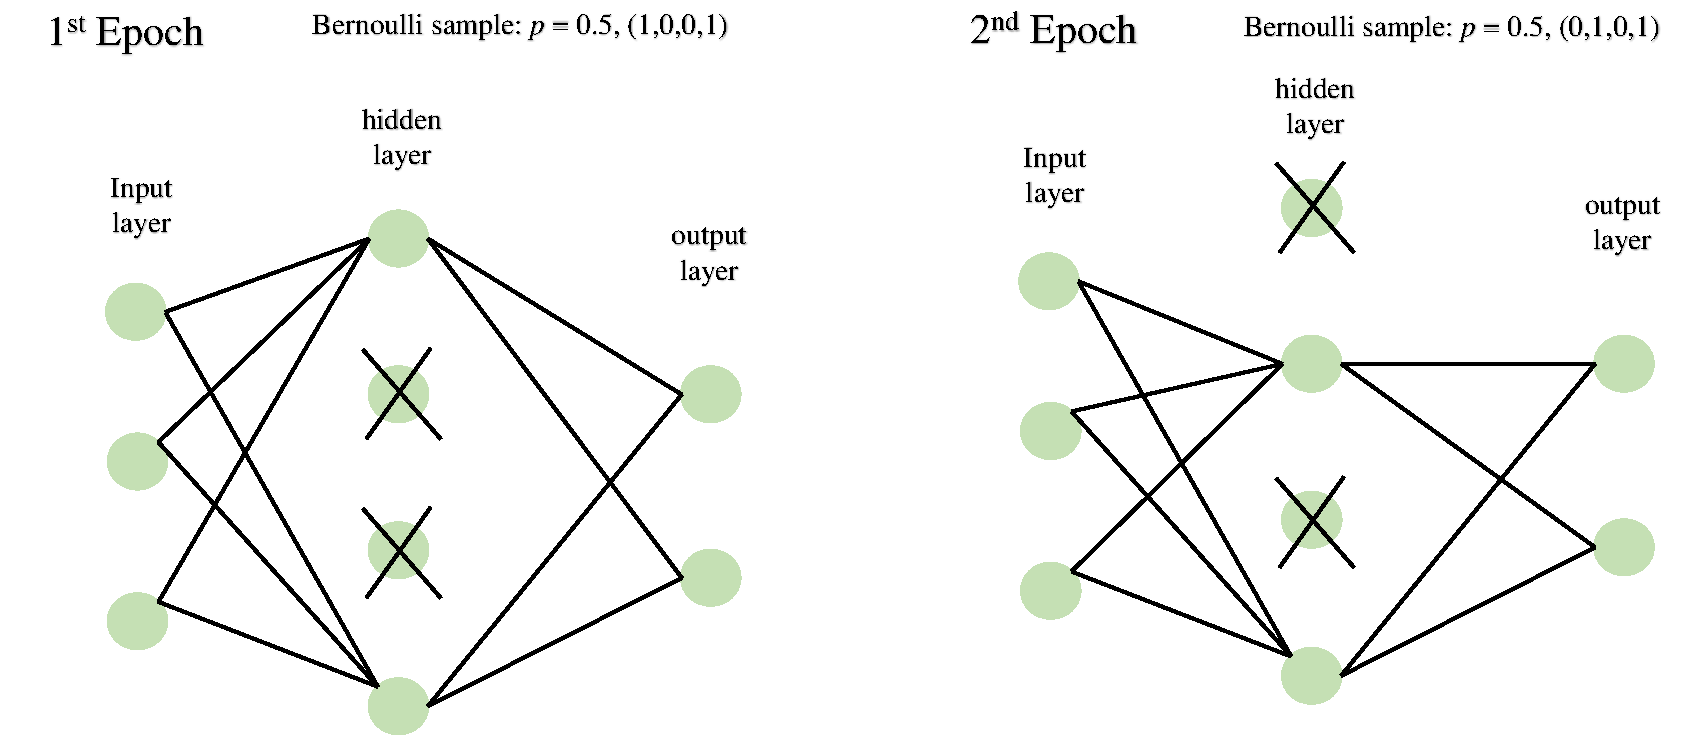
\includegraphics[width=1.0\textwidth]{dropout.pdf} %插入图片,[]中设置图片大小,{}中是图片文件名
\caption{The principle of how dropout works} %最终文档中希望显示的图片标题
\end{figure}
	

\end{frame}
%------------------------------------------------
\begin{frame}[allowframebreaks]
	\frametitle{Early stop method}
	The idea behind early stopping is to monitor the network's performance on a validation set during training and stop the training process once the validation error starts to increase, indicating that the network is starting to overfit the training data.

In the beginning, data set is separated into a training set and a validation set randomly. As the network is trained, the training error generally decreases over time, while the validation error initially decreases but then starts to increase again. This is because the network starts to overfit the training data, and the improvements in the training error do not generalize to new data.

\begin{figure}[H] %H为当前位置,!htb为忽略美学标准,htbp为浮动图形
\centering %图片居中
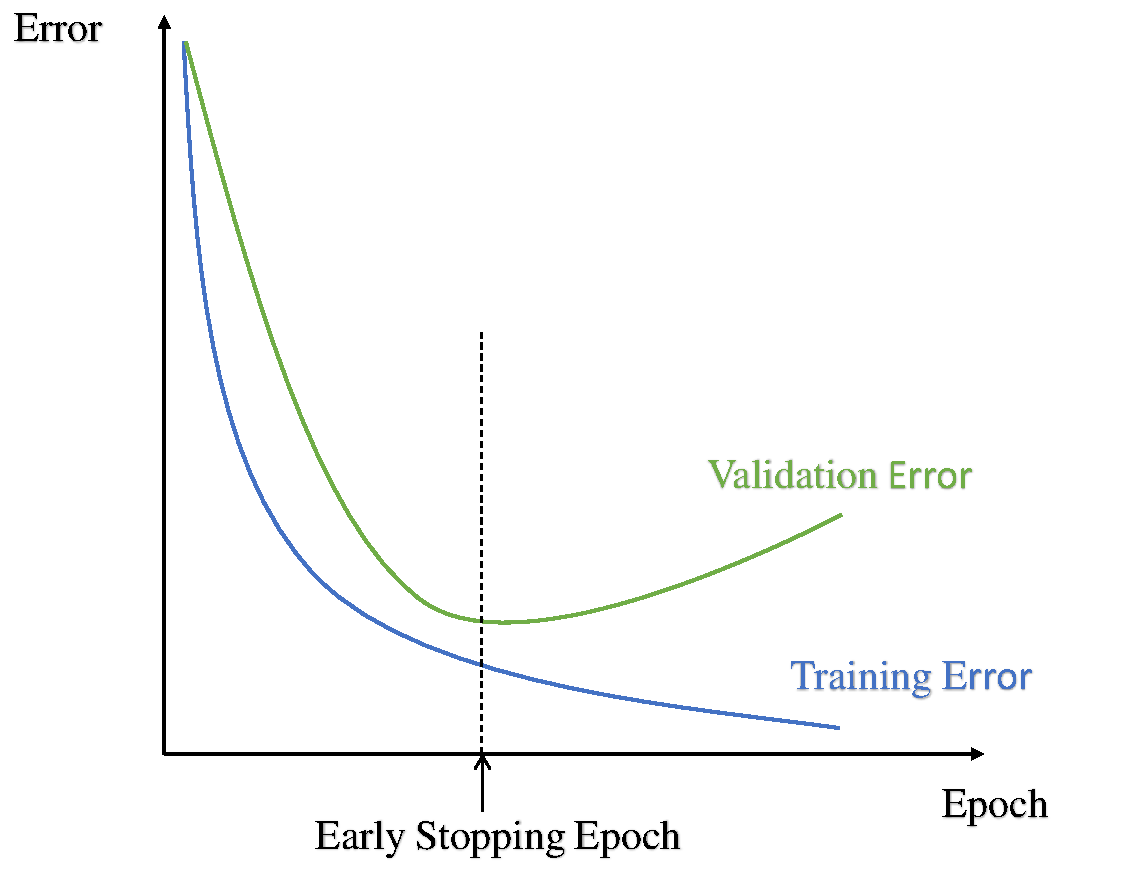
\includegraphics[width=0.5\textwidth]{earlystop.pdf} %插入图片,[]中设置图片大小,{}中是图片文件名
\caption{The principle of how early stop works} %最终文档中希望显示的图片标题
\end{figure}

The early stopping point is indicated by the dashed line in the graph. This is the point at which the validation error is at its minimum. At this point, the network has achieved the best possible generalization performance on the validation set. Any further training would cause the network to overfit the training data, resulting in worse generalization performance. Therefore, the training process is stopped at the early stopping point, and the network parameters at this point are used as the final trained model. This model has achieved the best possible generalization performance on the validation set and can be used to make predictions on new data.
	

\end{frame}

\end{document} 